\chapter{超声心动图切面的自动识别方法}
\label{chap:classification}

在心脏病常规临床检查中,二维实时超声心动图常用于评测心脏的结构和功能。临床超声检查通常主要包括三个步骤:探头扫描不同位置,选取标准切面和对标准切面的测量和诊断\citep{Chen2015}。其中,医师总结出来能更好辅助分析心脏功能结 构的特定位置和角度的超声心动图称为标准切面,其正确快 速选取不仅对临床诊断具有至关重要的意义,也为病例研究 提供比较依据。标准切面的自动识别是超声心动图智能分析和测量的基础。与自然图像相比,医学超声成像质量差,存在斑点噪声和伪影;并且各标准切面类内、类间差异大,使得标准切面的识别成为一个非常具有挑战性的问题。 

目前的研究主要集中在利用机器学习和图像处理等方法,进行超声心动图的自动识别、检索及切面内组织结构的定位和分割等。针对超声心动图的自动识别,2004年Shahram 等\citep{Ebadollahi2004}首次提出采用马尔科夫随机场,设计通用腔室模板检测 心脏腔室来辅助三类标准切面识别,但需额外信号来指定处 于舒张末期(End–Diastolic,ED)的切面。同样利用处于ED的标准切面,Kevin等\citep{KevinZhou2006}基于多类别提升算法框架,提取哈尔矩形特征训练弱分类器,同样需要检测心脏腔室的空间位置,辅助四类标准切面识别。基于降低特征维度的两层级联方法,把标准切面分类成心尖和胸骨旁两大类,然后进一步区分四类标准切面视频\citep{Otey2006,Roy2006b}。在文献\citepns{Ebadollahi2004}工作基础上整合局部和全局模板特征,利用多类逻辑提升分类算法,并指出能扩展到任意标准切面\citep{Park2007a}。在对心脏的循环跳动的时空信息进行统计分析的基础上,利用主动外观模型对形状和纹理进行建模,统计追踪一个心动周期并投影到运动空间进行分类\citep{Beymer2008},该方法处理的视频序列。把标准切面视为不同场景,提取低层全局特征来表征不同切面,利用改进核支持向量机进行分类\citep{Wu2014c}。这些方法可以归纳为两个阶段:首先根据先验人为设计特征来表征图像;然后利用机器学习中不同分类方法对特征向量进行建模分析得到分类器。然而受限于‘语义鸿沟’问题,根据特定先验人为设计特征,如大多数方法都针对心动周期的某个特定时刻的切面(如ED),会导致模型泛化性能差。

近来,深度卷积神经网络(Convolutional Neural Network,CNN)在大规模自然图像数据集(如ImageNet\citep{Russakovsky})上,识别性能远超传统方法\citep{Krizhevsky2012}。主要得益于深度学习利用大量标注数据从图像原始像素出发,逐层分级学习中高层的抽象语义特征\citep{Sharif2014}。
当前实践中由于深度学习需要大量的标注数据,所以仅在少数医学任务中取得有限的成功应用,且对深度模型的鲁棒性和有效性也缺乏详尽分析。Chen等\citep{Chen2015}利用CNN结合领域知识,在胎儿超声心动图标准切面的自动识别问题中取得良好的识别效果,但胎儿跟成人超声心动图差异大,具有很大特殊性。Bar等\citep{Bar2015Chest}利用自然图像训练的模型对胸腔X-射线图像进行特征提取并结合全局特征\citep{Oliva2001}得到最优检测结果,并没有对特定医学数据进行迁移训练,仅是作为特征提取器。Margeta等\citep{Margeta2015}针对心脏核磁共振图像利用微调迁移从自然图像学习的模型,但没对模型有效性进行分析。

目前深度CNN模型的理论分析工作还不是很完善,能自动学习语义特征的工作机理还是个“黑箱”。对于不同的模型的比较除了准确率之外并没有很好的评价方法,优异的泛化能力从何而来仍是个开放问题。一些工作\citep{simonyan14deep,Mahendran2015,Zeiler2014,Zhou2015}通过可视化各层激活值和卷积核来更好理解深度CNN。对在给定数据集上训练得到的深度CNN网络模型,Simonyan等\citep{simonyan14deep}用反卷积来可视化每个神经元的最大激活值。Mahendran等\citep{Mahendran2015}通过对学习到的每层的特征编码进行反编码,建立每层特征编码和原图像的映射关系。Zeiler等\citep{Zeiler2014}试图通过梯度上升方法迭代寻找图像使得最大化激活某个或某些特定的神经元。神经元对图像每个像素的梯度描述了当前像素的怎样改变能影响分类结果。前三个方法均是对已训练的模型进行分析,而类激活映射图(Class Activation Maps,CAM)方法\citep{Zhou2015}用全局平均池化层代替全连接层改进训练过程,分类性能虽略有降低,但能指示出特定类别的显著性判别区域,能很好的解释模型的有效性。
本文提出一种基于深度CNN识别超声心动图的方法(Deep Echocardiogram,Deep-Echo):1)引入空间金字塔平均池化层代替全连接层,一方面大大减少模型参数,降低过拟合风险;另一方面网络结构变为全卷积网络,使得不用限制输入图像尺寸大小,这对医学超声图像更为重要。2)为验证该算法的鲁棒性和有效性,针对数据集进行详尽实验,研究分析了深度学习方法的高识别率和优异泛化能力的原因。
 
\section{Deep-Echo模型}

将分别从如何构建全卷积网络、全局空间金字塔平均池化层、将类别显著性图纳入可视化过程、如何扩增数据等方面介绍提出的Deep-Echo模型。
\subsection{全卷积的网络}

与GoogLeNet模型\citep{Szegedy2015}、ResNet模型\citep{he15}类似,使用多层卷积层(每层包括ReLU层、BN层和Pooling层),用全局平均池化操作替代全连接层。Deep-Echo模型结构中对最后卷积层输出的特征图,用金字塔平均池化层\citep{He2015spp}代替最大化池化层和全连接层。最后一层输出单元数目为类别的数目,由于实验采用的标准切面有七个类别,因此最后一层输出7,依次对应相应的类别,采用交叉熵损失函数加L2正则化。卷积核数目从64开始, 每经过一次最大池化层,卷积核数目翻倍,直到512为止。学习率初始化为0.01。具体实验步骤和参数设置见后文实验部分。整个网络结构如图\ref{fig:ch03_02}所示。
 \begin{figure}[!htbp]
\centering
%trim option's parameter order: left bottom right top
%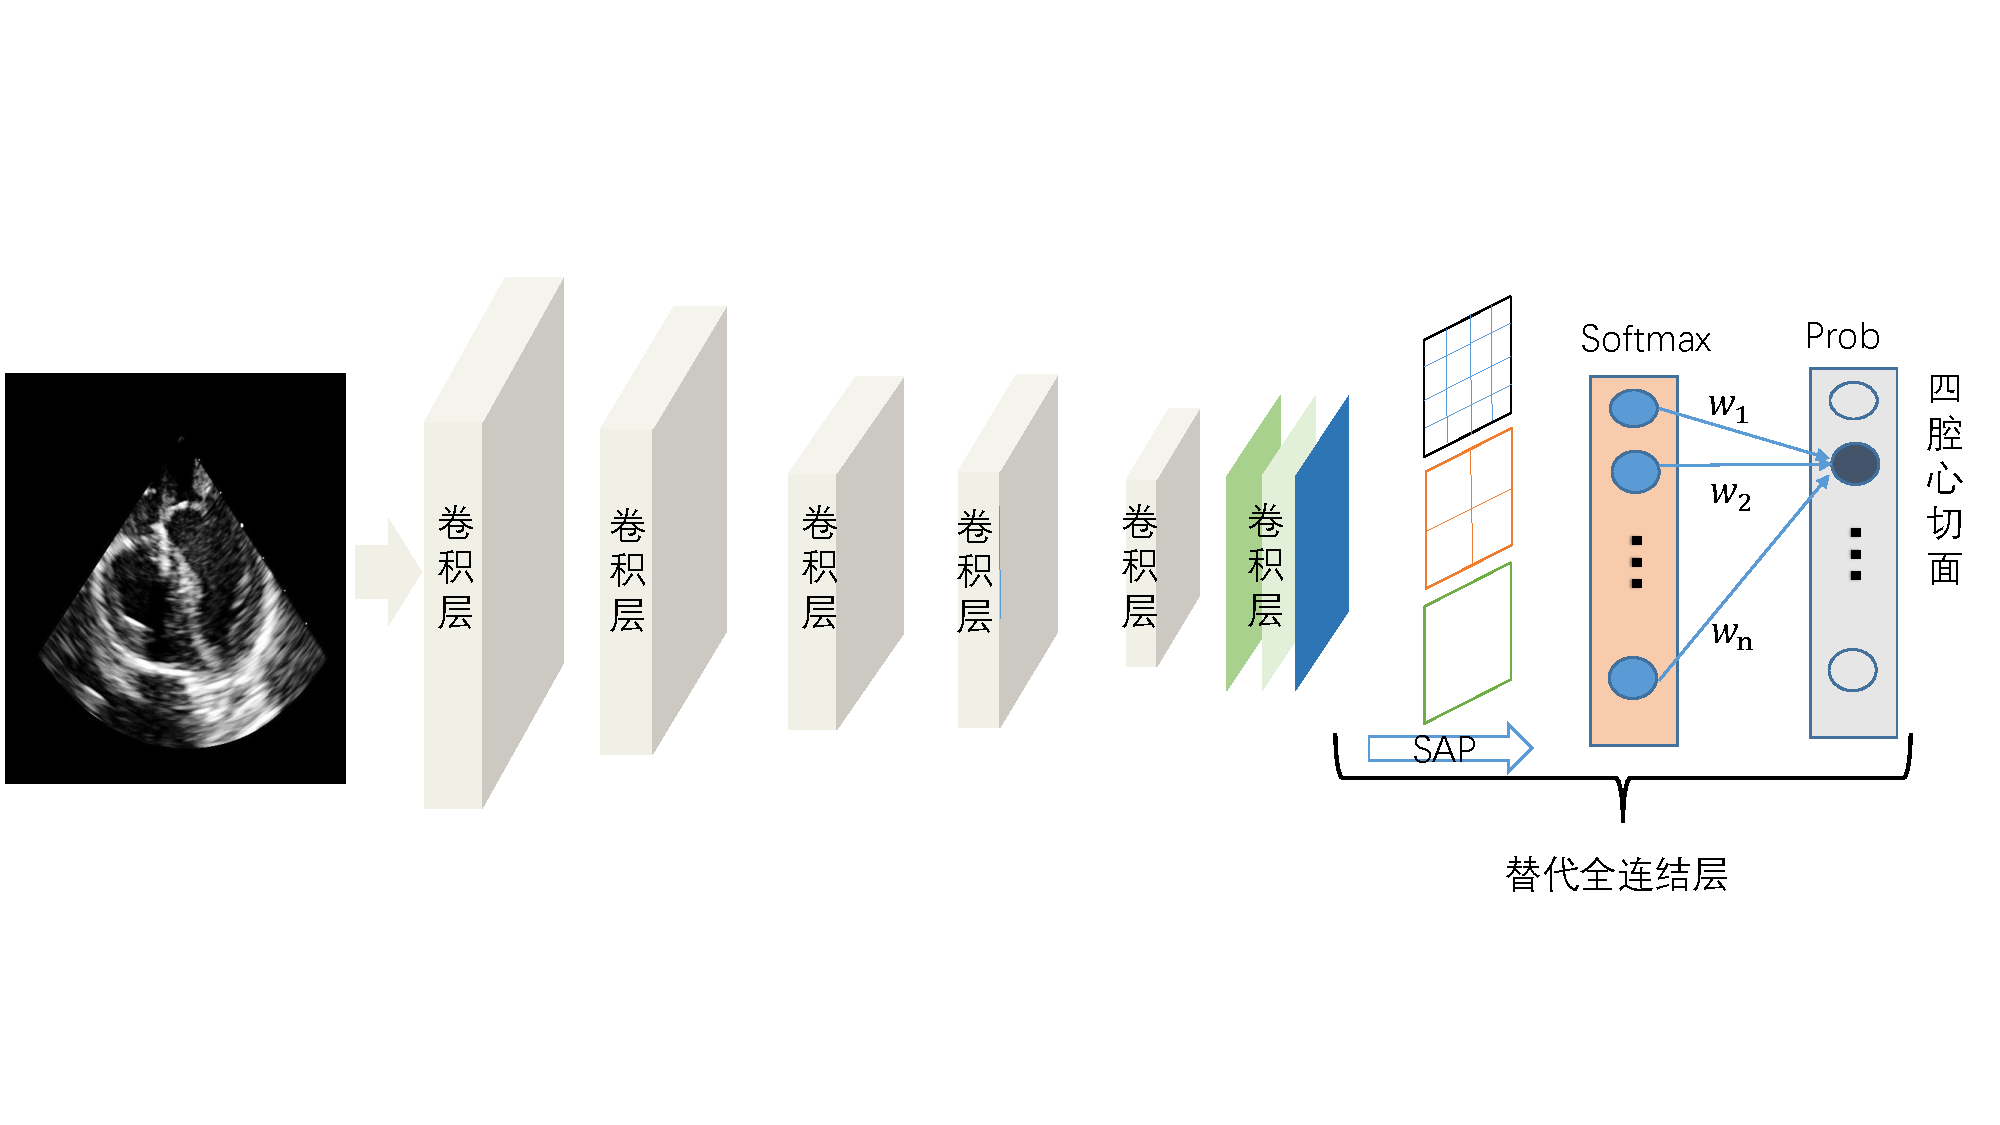
\includegraphics[trim = 30mm 0mm 30mm 0mm, clip, width=0.45\textwidth]{ch03_02}
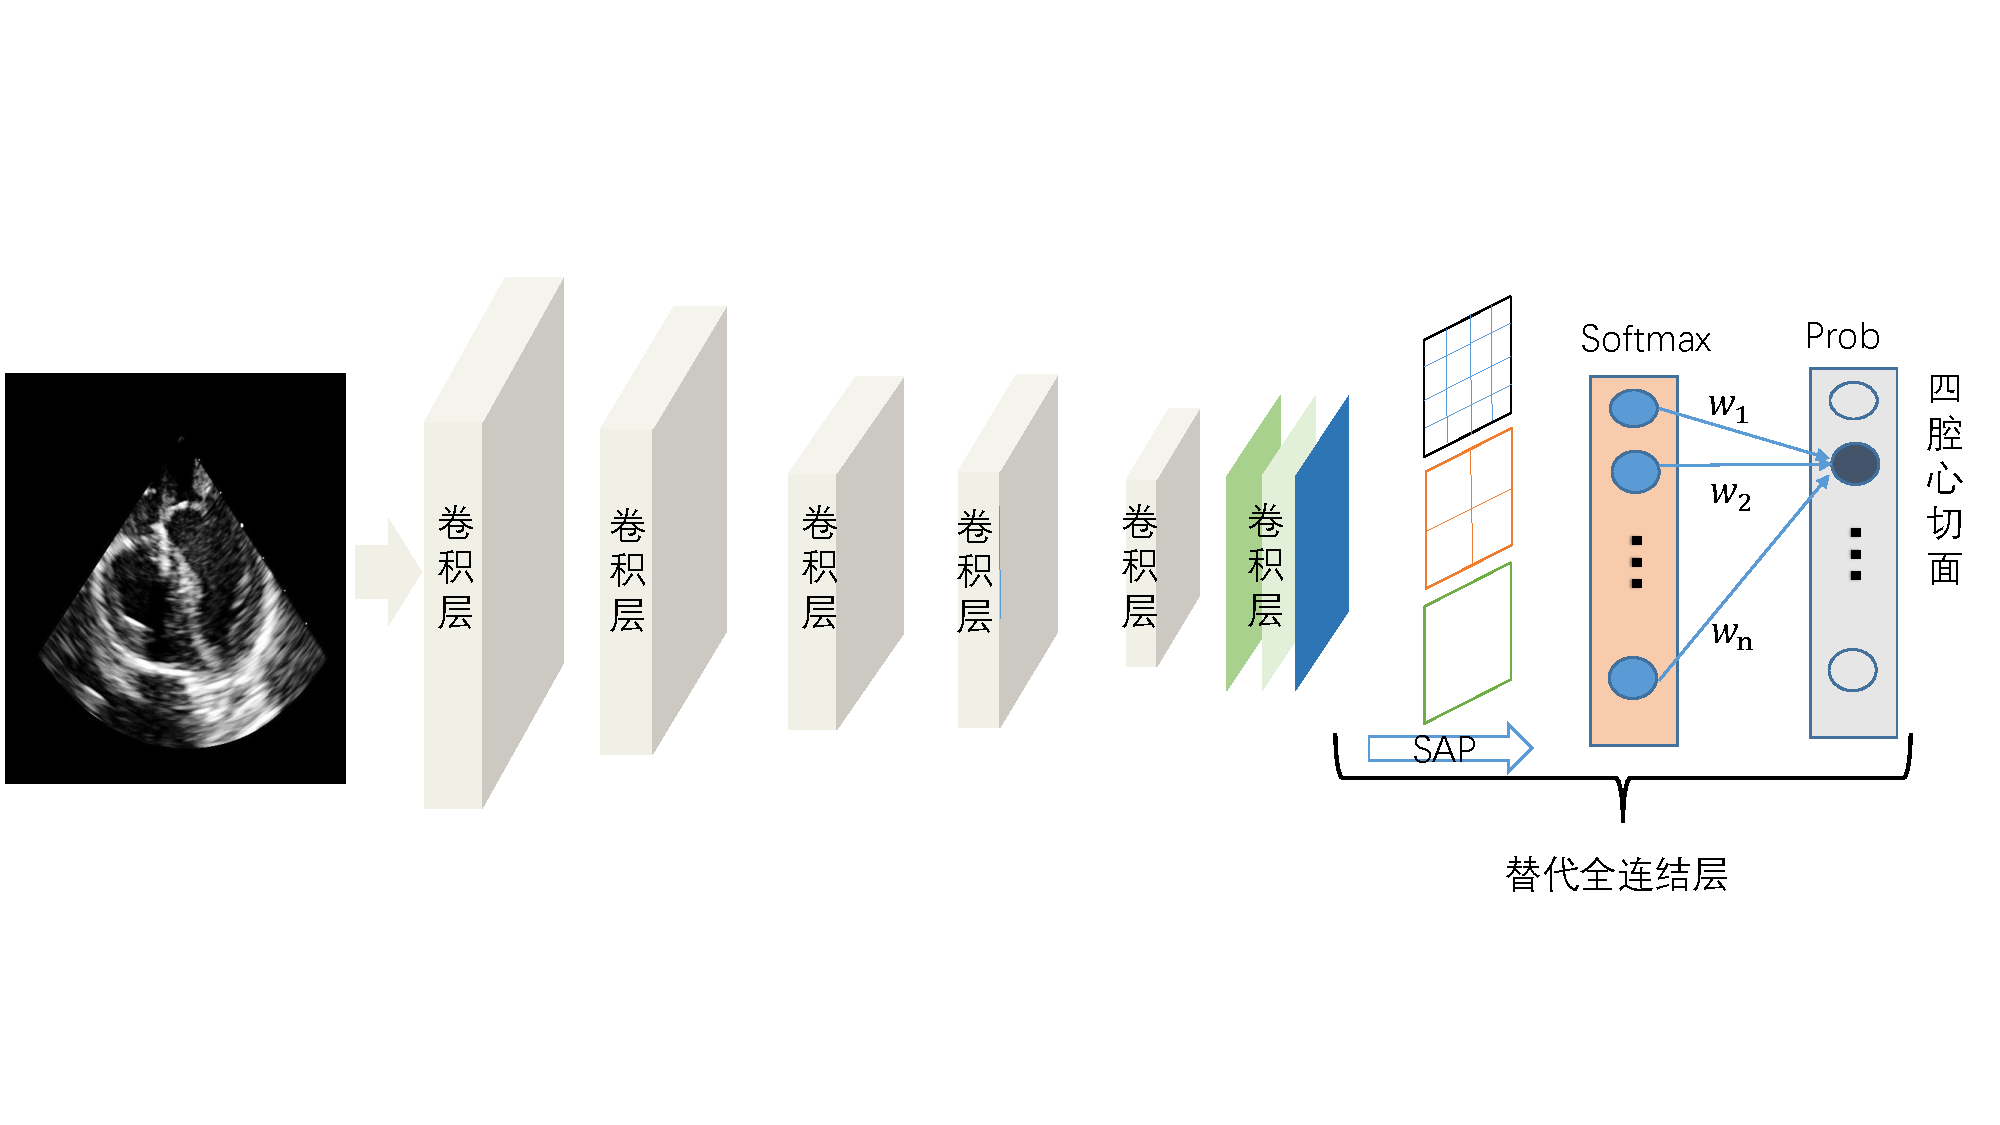
\includegraphics[width=0.85\textwidth]{ch03_02}
\caption{Deep-Echo模型结构示意图}
\label{fig:ch03_02}
\end{figure}

\subsection{空间金字塔均值池化层}

针对深度CNN模型中全连接层的两个缺点:全连接层丢失了空间信息,限制了 CNN 只能接受固定尺度的输入, 一般只能通过图像尺度归一化的方法来处理不同尺度的输入图像,且使得模型可视化变得不可解释;全连接层参数拥有大约90\%的模型参数,如AlexNet模型\citep{Krizhevsky2012}和VGG16模型\citep{Chatfield2014}中全连接层参数占全部参数分别为38M/61M和103M/138M,从而导致模型更容易过拟合\citep{Szegedy2015}。
为解决这两个问题,He等提出空间金字塔池化 (Spatial Pyramid Pooling, SPP)方法\citep{He2015spp}。 SPP通过使用多个不同大小的池化操作保证固定的特征向量输出,从而允许 CNN 接受任何尺度的输入, 增加了模型的尺度不变性, 抑制过拟合。与传统的全连接层不同,对每个特征图一整张图片进行多尺度的空间金字塔均值池化,这样每张特征图都可以得到多个尺度的输出。本文方法跟空间金字塔池化网络类似都是三个尺度的空间金字塔池化(1×1, 2×2, 4×4),其差异在于后不再接多个全连接层,同时用平均池化代替最大化池化,目的在于方便可视化模型的空间位置信息。
\subsection{微调迁移学习}

   利用深度学习进行超声心动图的标准切面识别,仍存在针对小数据量直接训练是否会出现过拟合问题;能否跨领域进行迁移学习,即在自然图像数据集上训练得到的模型能否微调应用到跨领域的超声心动图上。文献\citepns{Zhou2015}中指出,用全局平均池化代替全连接层直接随机初始化,从头开始训练模型收敛困难且分类性能下降,故对现有模型进行改造,即针对在自然图像集上预先训练得到的模型如,Alexnet模型等,变换最后的输出层为所述金字塔平均池化结构,调小学习率后在超声心动图标准切面数据上进行微调迁移学习。
训练时,由于超声心动图的特殊性,人工标注费时费力,对数据集进行扩增能降低人工标注的需求。但扩增数据需注意不能打乱标准切面图像内在的局部结构,因此对切面数据只进行水平镜像翻转和旋转。通过引入BN归一化层能减轻对Dropout的依赖,提高泛化能力,并且本文直接去掉全连接层,故并未采用Dropout技术。
迁移学习时,由于深度模型中低层的卷积核是跟人类视觉的初级细胞很类似,因此是可以直接迁移复用,高层要针对目标学习判别性信息需进行重新学习\citep{Zhou2015}。针对超声心动图的实验支持这样的结论,不同模型的分类准确率都很高,具体实验见后文实验部分。但对于计算机医学辅助诊断而言,模型怎样决策判断比分类准确率更重要。即需解释模型为什么有效和优异的泛化能力从何而来。
\subsection{类别显著激活映射图}

 前文所提模型能高效提取超声心动图标准切面的特征,对超声心动图的单扇形和双扇形标准切面都能很好的识别,甚至对互联网上随意选取的标准切面也能识别。但对模型的有效性和解释性缺乏有力分析,使得对模型决策判断的可信性产生怀疑。
针对超声心动图,采用\citepns{Zhou2015}提出可视化分析的方法,将其和空间金字塔平均池化结合。对给定图像, $f_{j}(x,y)$ 表示卷积层(x,y)位置上第j个神经元的激活值,对第j神经元的平均池化操作结果对给定类别k的得分函数S:
\begin{equation} \label{eq:s}
     S_{k}=\sum_{j}w_{j}^{k}\sum_{x,y}f_{j}(x,y)
\end{equation}	    
其中 $w_{j}^{k}$ 是第j 个神经元和第k 类的连接权重,后接多类多元逻辑损失层,然后由公式\ref{eq:m}可得定义类别激活映射图:	
  	      \begin{equation} \label{eq:m}
     M_{k}=\sum_{j}w_{j}^{k}f_{j}(x,y)
\end{equation}
其中,$M_{k}$ 表明在空间(x,y)的激活值对该类别分类结果影响的重要性。对类别激活映射图直接双线性插值得到与原图大小相等的显著性图。本文将其和多尺度空间金字塔平均池化结合,得到对多个空间尺度的类别显著激活映射图。值得注意的是,对不同的尺度可设置不同的权重,本文采用同等权重进行融合。该图是对图像空间显著性区域的置信度判别,能辅助可视化分析深度模型的决策过程,在一定程度上解释模型可效性。

\section{实验结果和分析}
\subsection{实验数据选取和实验方法}

本文实验数据来自四川大学华西医院,为临床检查中的经食道超声心动图。所选切面视频包含单扇形和多普勒成像的双扇形两种,其中对双扇形的切面视频,仅取不包含彩色多普勒成像的切面(如图\ref{fig:ch03_03}所示)。经专业医师标注的标准切面视频中,至少包含2-3个心动周期,并依据医师建议从视频中截取包含一个心动周期的10帧图像,并经医师检验筛选后得到最终数据集。
\begin{figure}[!htbp]
\centering
%trim option's parameter order: left bottom right top
%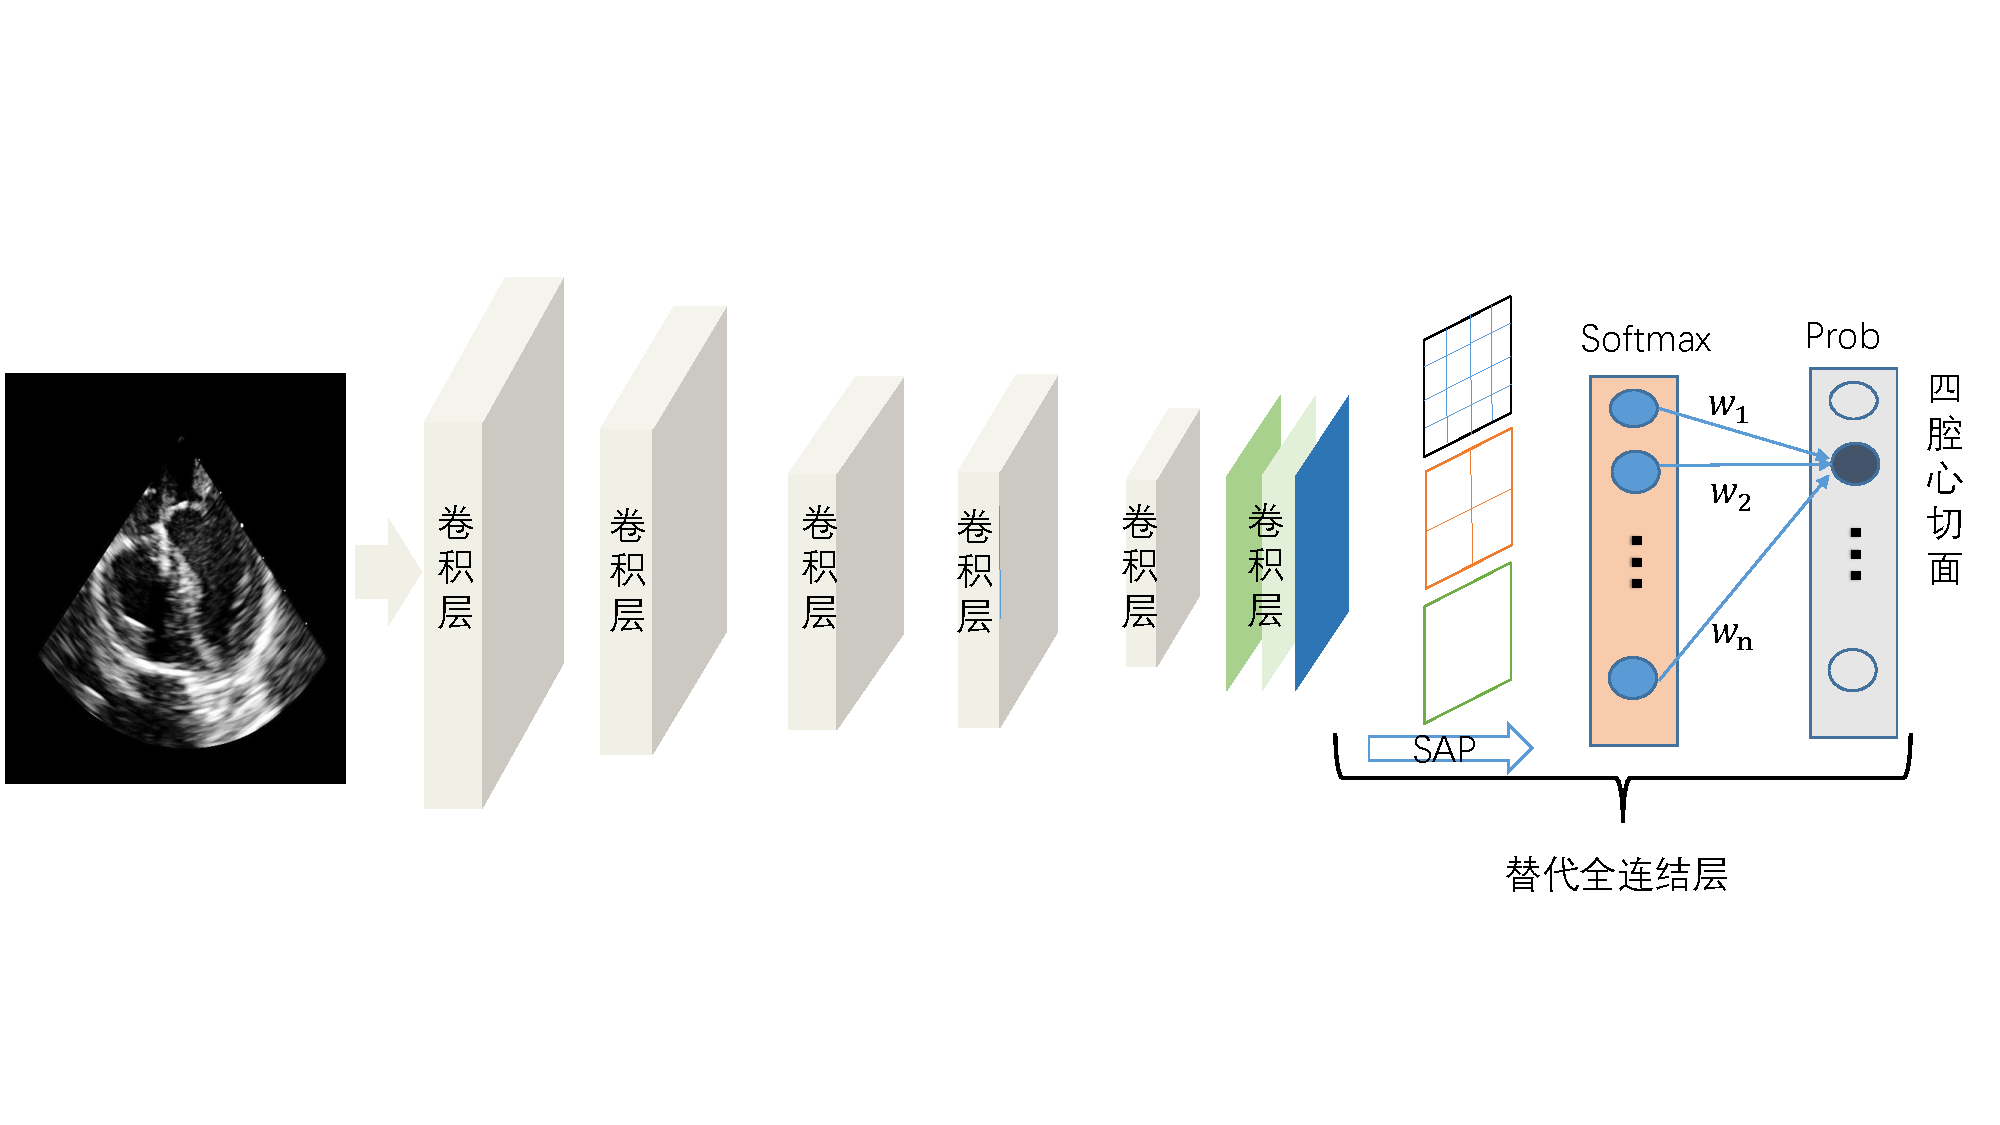
\includegraphics[trim = 30mm 0mm 30mm 0mm, clip, width=0.45\textwidth]{ch03_02}
\includegraphics[width=0.85\textwidth,height=0.4\textheight]{ch03_03}
\caption{七类标准切面超声心动图及数量分布}
\label{fig:ch03_03}
\end{figure}

试验中所用标准切面类别和数量分如布图\ref{fig:ch03_03}所示。依据探头在食管中段(ME)和经胃底(TG)的位置和角度不同,在图\ref{fig:ch03_03}中7类标准切面分别为:a为升主动脉长轴(AescLAX) ,b为主动脉瓣长轴(MEAVLAX),c为主动脉瓣短轴(MEAVSAX),d为降主动脉长轴(descLAX),e为降主动脉短轴(descSAX),f为食管中段四腔心(ME4C),g为经胃底心室短轴(TGLAX)。其中,d,e,g为单扇形切面,其余为双扇形中截取的切面。训练集(17932张)和测试集(2217张)由不同时期采集不同病人对象数据的随机划分。值得注意的是,所有数据都经过裁剪操作以隐去患者信息。
\subsection{识别实验结果和分析}

	本文在构建的超声心动图的数据集上测试分类性能。采用Caffe框架\citep{Jia2014}实现深度卷积网络结构, 预训练模型来自Caffe model zoo。使用具有Intel®Core TM i5 3.2GHz处理器和12GB内存的Tian X GPU测量所需的时间,单个切面所需的分类识别时间平均需要10毫秒,基本可满足实时识别。
为验证从自然图像训练的模型能迁移到经食道超声心动图上,输入图像归一化为256x256,网络初始学习率设为0.001,迭代一定轮数动态调整学习率大小,其他参数的设置跟原文献中训练网络结构时一致。 三种不同网络结构的深度模型微调前后在同一测试集上的准确率随着迭代次数的增加最后趋于一致,如表\ref{tab:ch03_01}所示,Scratch表示不经过微调,Finetune表示经过微调。Deep-echo模型结构跟AlexNet模型类似,是在其结构基础上去掉全连接层,用空间金字塔池化层代替,比VGG16和GoogLeNet模型的层数更少,模型结构更简单,而分类准确率却接近,表明提出方法的有效性。针对VGG16模型和Google Net模型也可同样设置,本文主要关注点不是得到分类精度最优的分类模型,故并未全部加以实验验证。
\begin{figure}[!htbp]
\centering
%trim option's parameter order: left bottom right top
%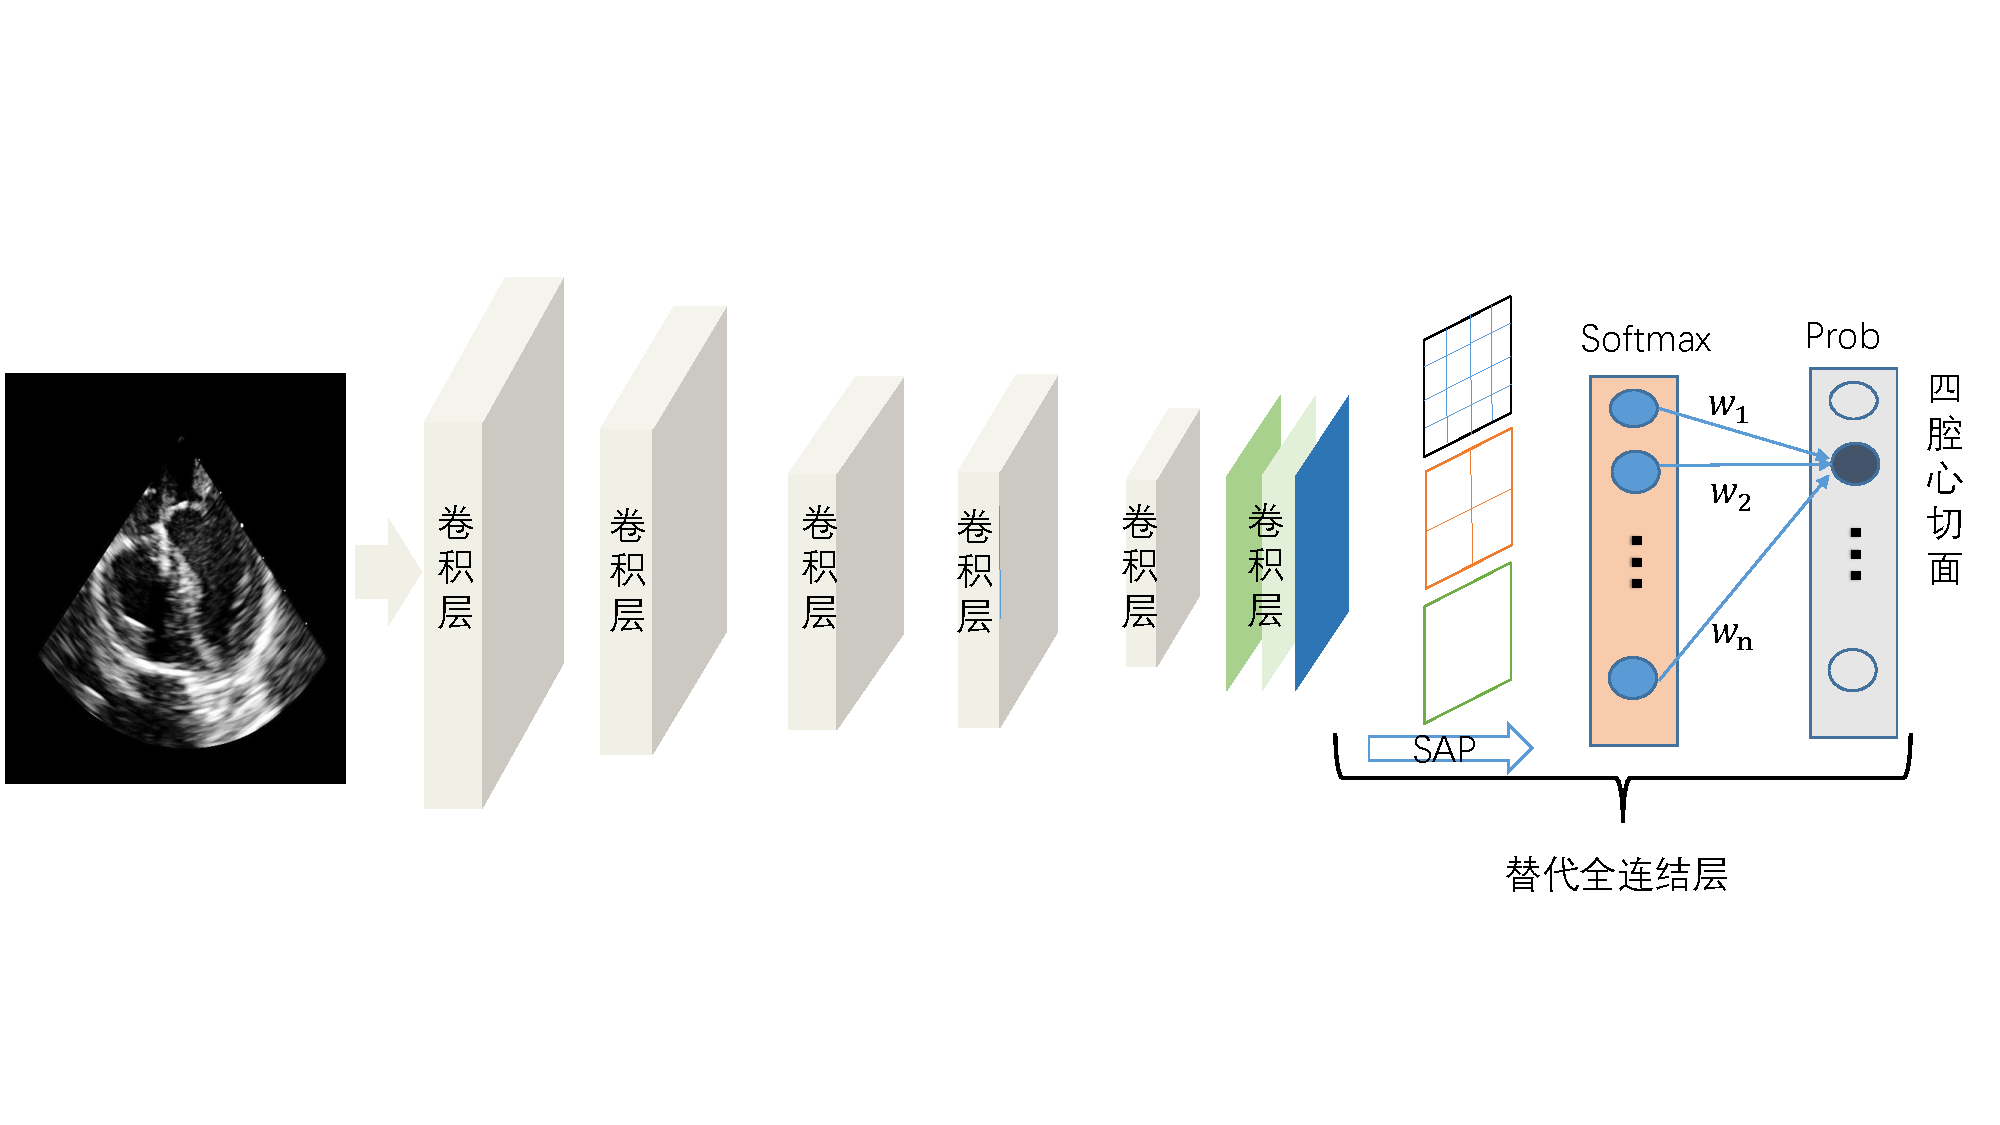
\includegraphics[trim = 30mm 0mm 30mm 0mm, clip, width=0.45\textwidth]{ch03_02}
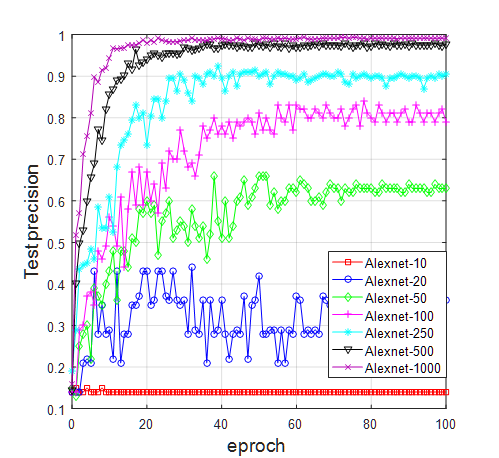
\includegraphics[width=0.85\textwidth]{ch03_04}
\caption{不同数据量的平均分类精度}
\label{fig:ch03_04}
\end{figure} 
为验证训练集数据量对深度卷积网络的影响。网络结构采用AlexNet模型结合空间金字塔池化层,在不同数据量上微调,实验结果如图\ref{fig:ch03_04}所示,数字代表每类至多的数目,随着数据量的增加,模型准确率随之提升,可知针对超声心动图标准切面识别问题,并不用构建很大的数据集进行识别,如图\ref{fig:ch03_03}中每类至多500达到的平均准确率接近使用全部训练集的结果。可推断采用微调技术,能显著减少深度模型对大数据量的依赖。
\begin{table}[!htbp]
    \centering
    \footnotesize% fontsize
    \setlength{\tabcolsep}{4pt}% column separation
    \renewcommand{\arraystretch}{1.2}%row space 
    \begin{tabular}{lcccccccc}
        \hline\hline
          \multicolumn{2}{c}{\ \ \ \ \ \ \ \ 平均分类精度比较} \\
        \cline{2-3}% partial hline from column i to column j
           \qquad  & Scratch & Finetune \\
        \hline
        AlexNet & $93.35\%$ & $93.68\%$ \\
        \hline
        VGG16 & $96.66\%$ & $96.81\%$ \\
        \hline
        GoogleNet & $97.36\%$ & $97.42\%$ \\
        \hline
        Deep-Echo & $\textbf{97.49\%}$ & $\textbf{99.12\%}$ \\
        \hline\hline
    \end{tabular}
    \caption{不同模型分类精度比较}
    \label{tab:ch03_01}
\end{table}


为了验证最优模型在不同类别的分类性能,7分类的混淆矩阵如图\ref{fig:ch03_04}所示,每行代表实际的类别标签,每列代表预测的标签。最终的平均分类精度为97.49\%。分类置信度较低的是升主动脉长轴(AescLAX),其他各类的准确率都较高。

\subsection{模型可解释性实验结果分析}
深度卷积网络能在标准切面识别问题上得到较高的分类精度,但仅从分类准确率上评价模型存在局限性。为分析模型的有效性,采用文中所述可视化方法,对迁移后的Deep-echo模型进行实验。
\begin{figure}[!htbp]
\centering
%trim option's parameter order: left bottom right top
%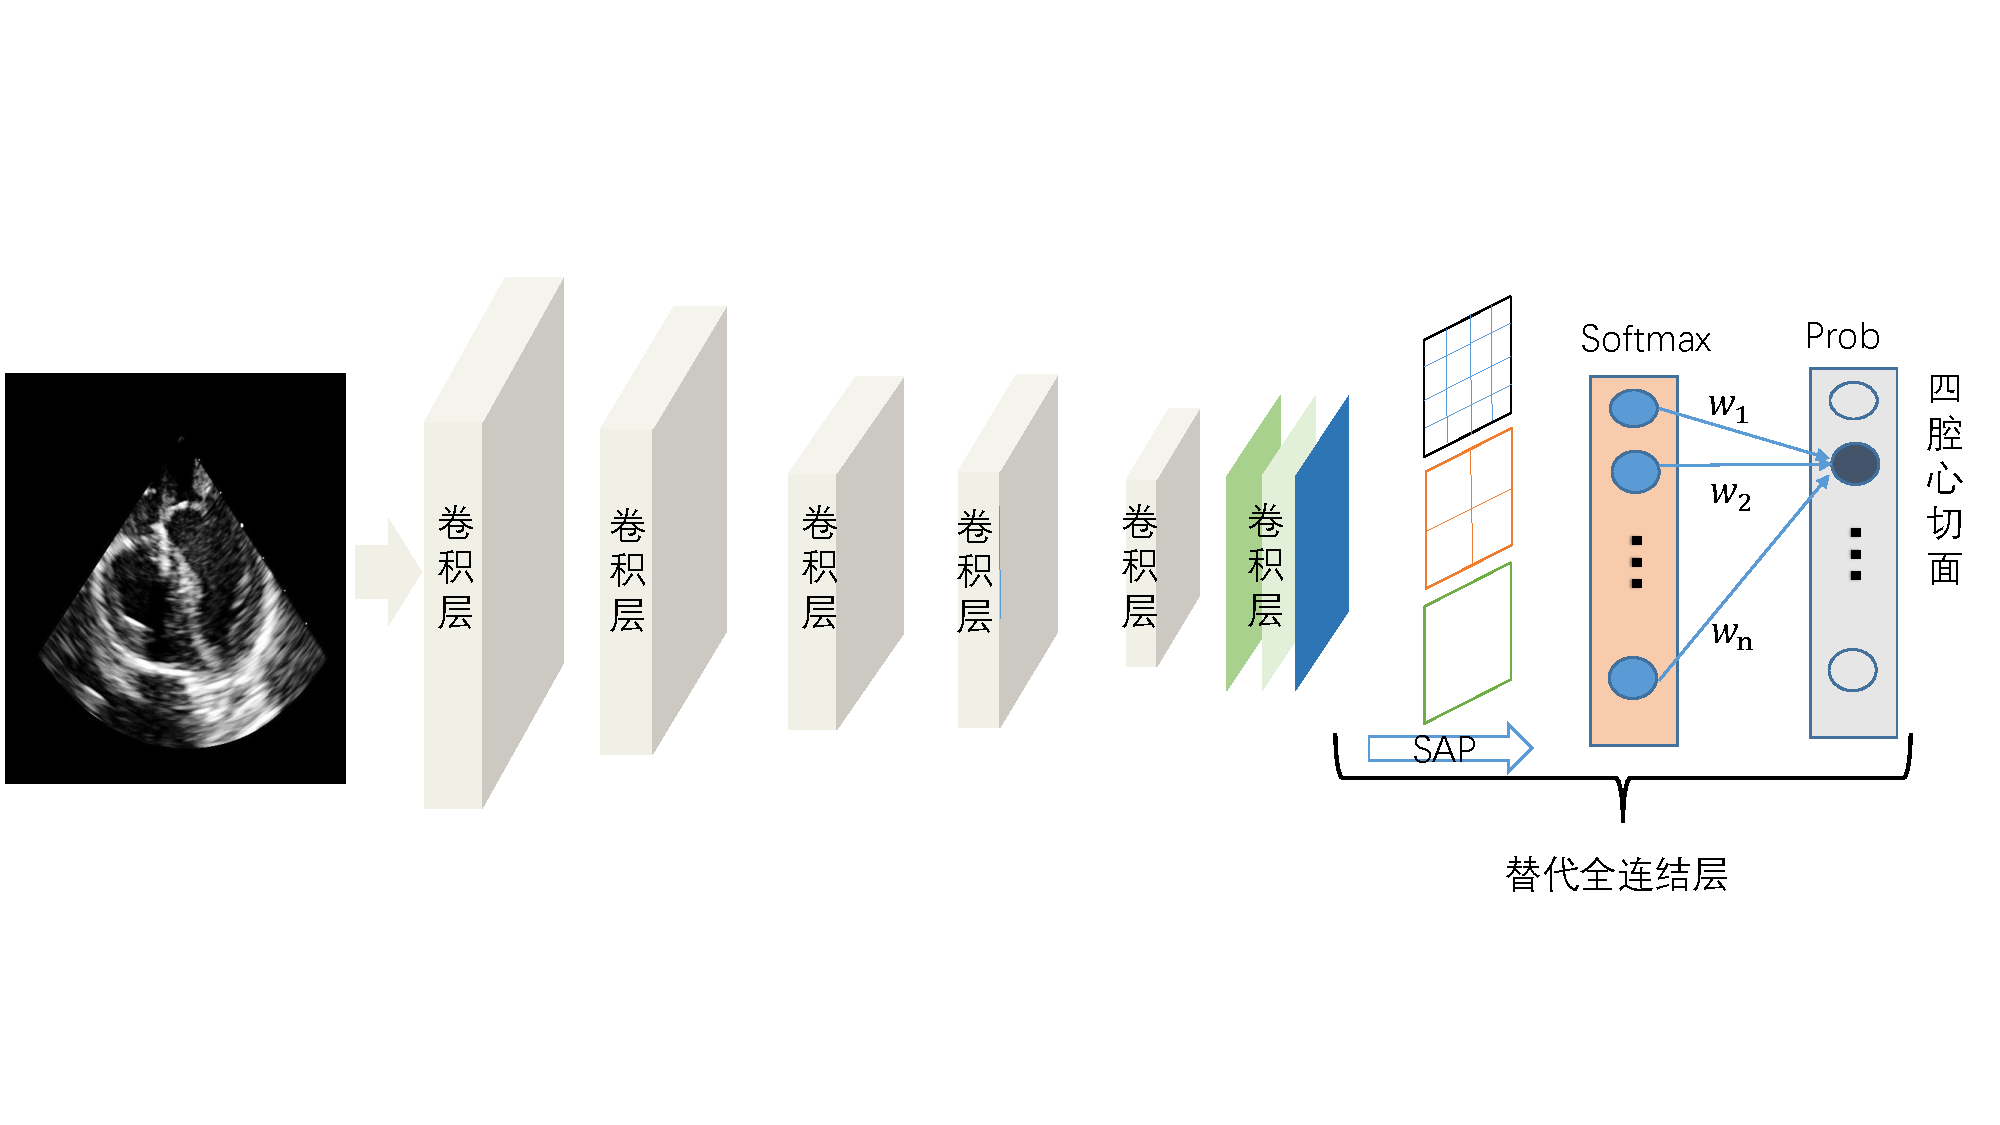
\includegraphics[scale=0.6,trim = 30mm 0mm 30mm 0mm, clip, width=0.45\textwidth]{ch03_02}
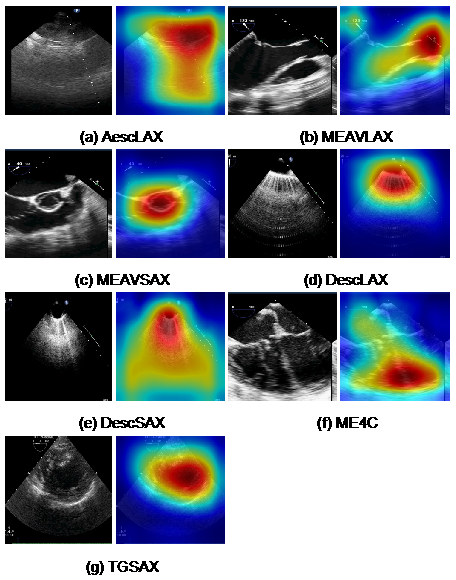
\includegraphics[width=0.85\textwidth,height=0.4\textheight]{ch03_05}
\caption{各类切面的原图和显著性热力图}
\label{fig:ch03_05}
\end{figure}  
 
实验结果如图\ref{fig:ch03_05}各类切面的原图和显著性热力图所示,图中为各类切面和对应的类别显著性热力图。类别显著性图中的颜色从蓝到红,表示原图像素中对分类结果影响的重要性是从轻到重。图中结果能很好的解释模型的有效性,并且跟专业医师的判断一致,如图\ref{fig:ch03_05}c中显著性热力图红色区域图定位到图中的圆圈;图\ref{fig:ch03_05}d中定位到的干涉条纹;图\ref{fig:ch03_05}f定位到左心室和右心室的边界等;都跟医师的决策判断依据是一致的。
\begin{figure}[!htbp]
\centering
%trim option's parameter order: left bottom right top
%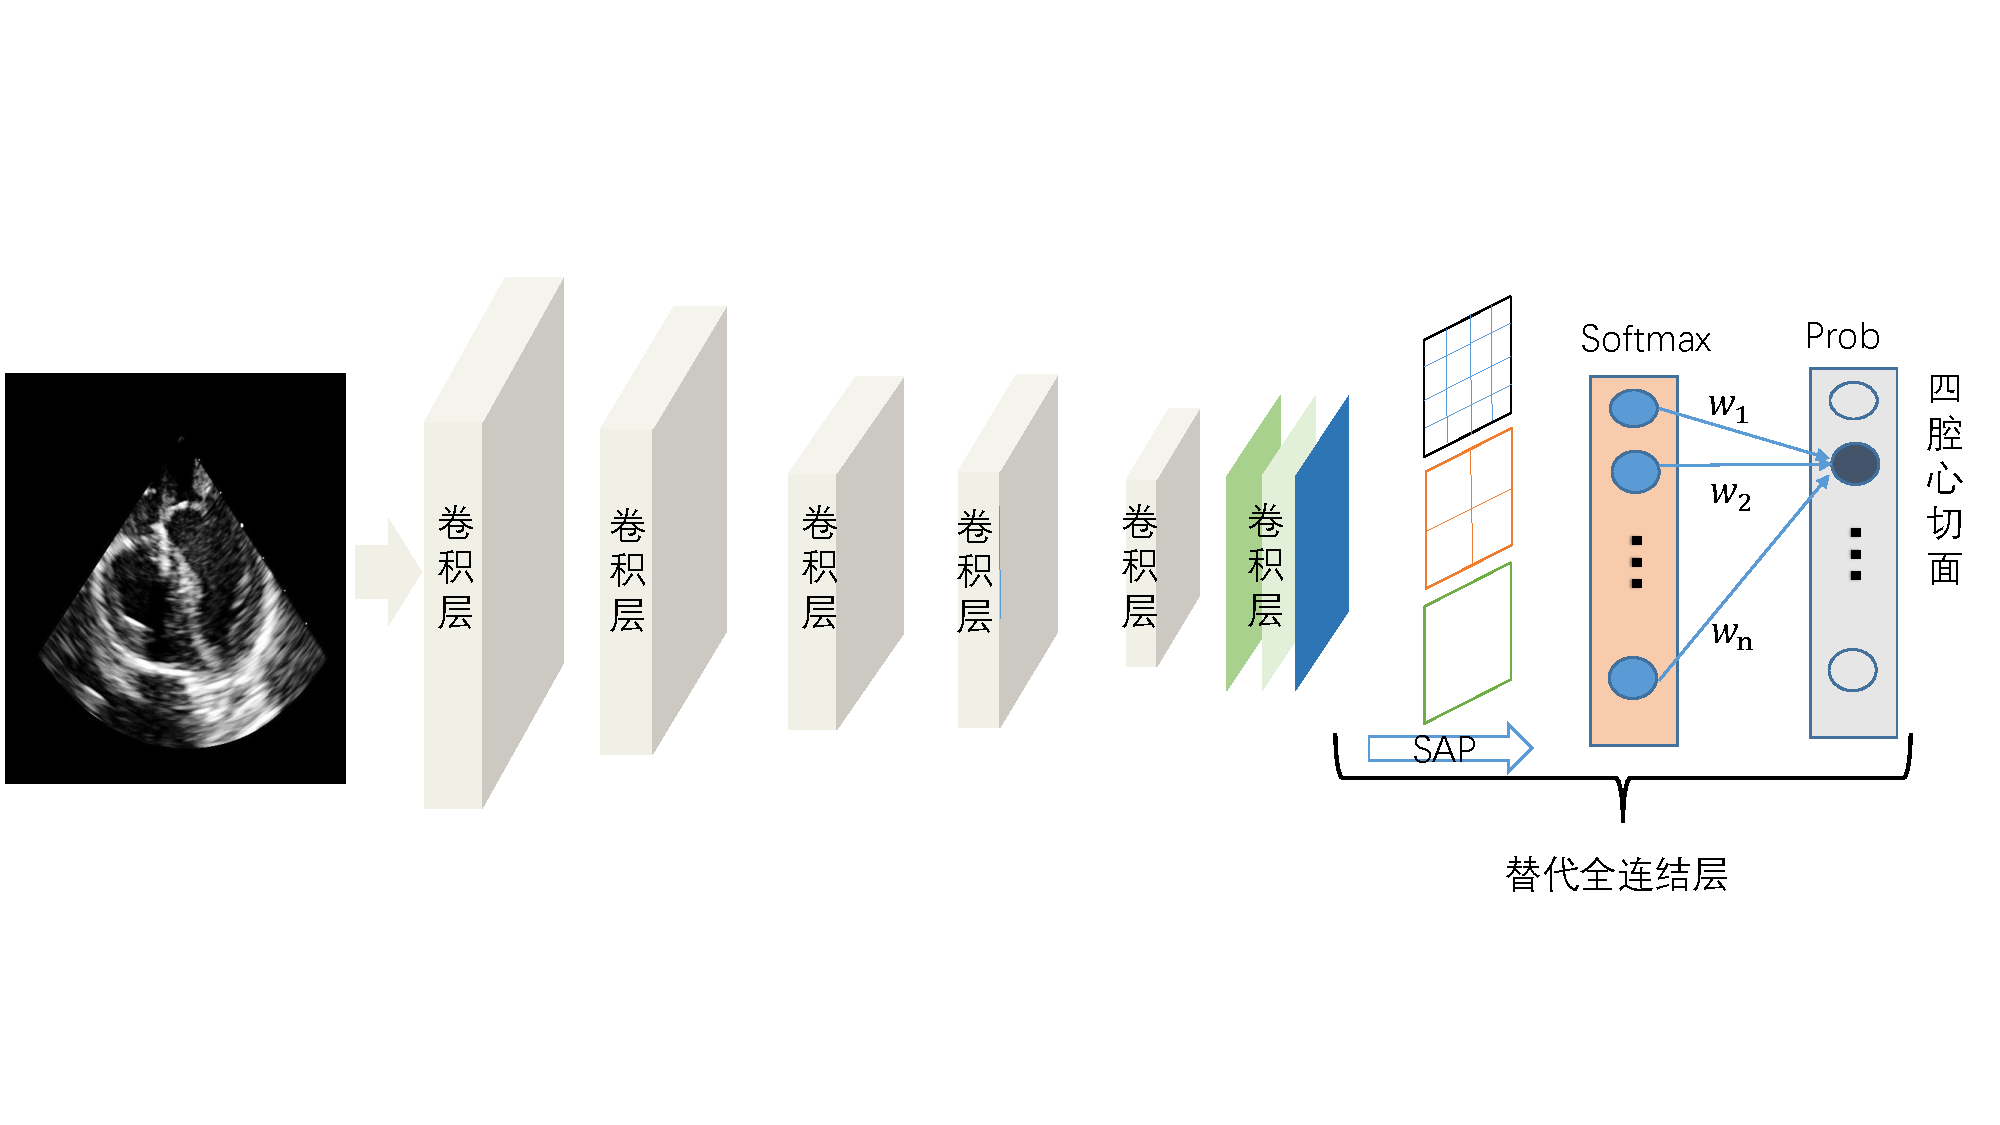
\includegraphics[scale=0.6,trim = 30mm 0mm 30mm 0mm, clip, width=0.45\textwidth]{ch03_02}
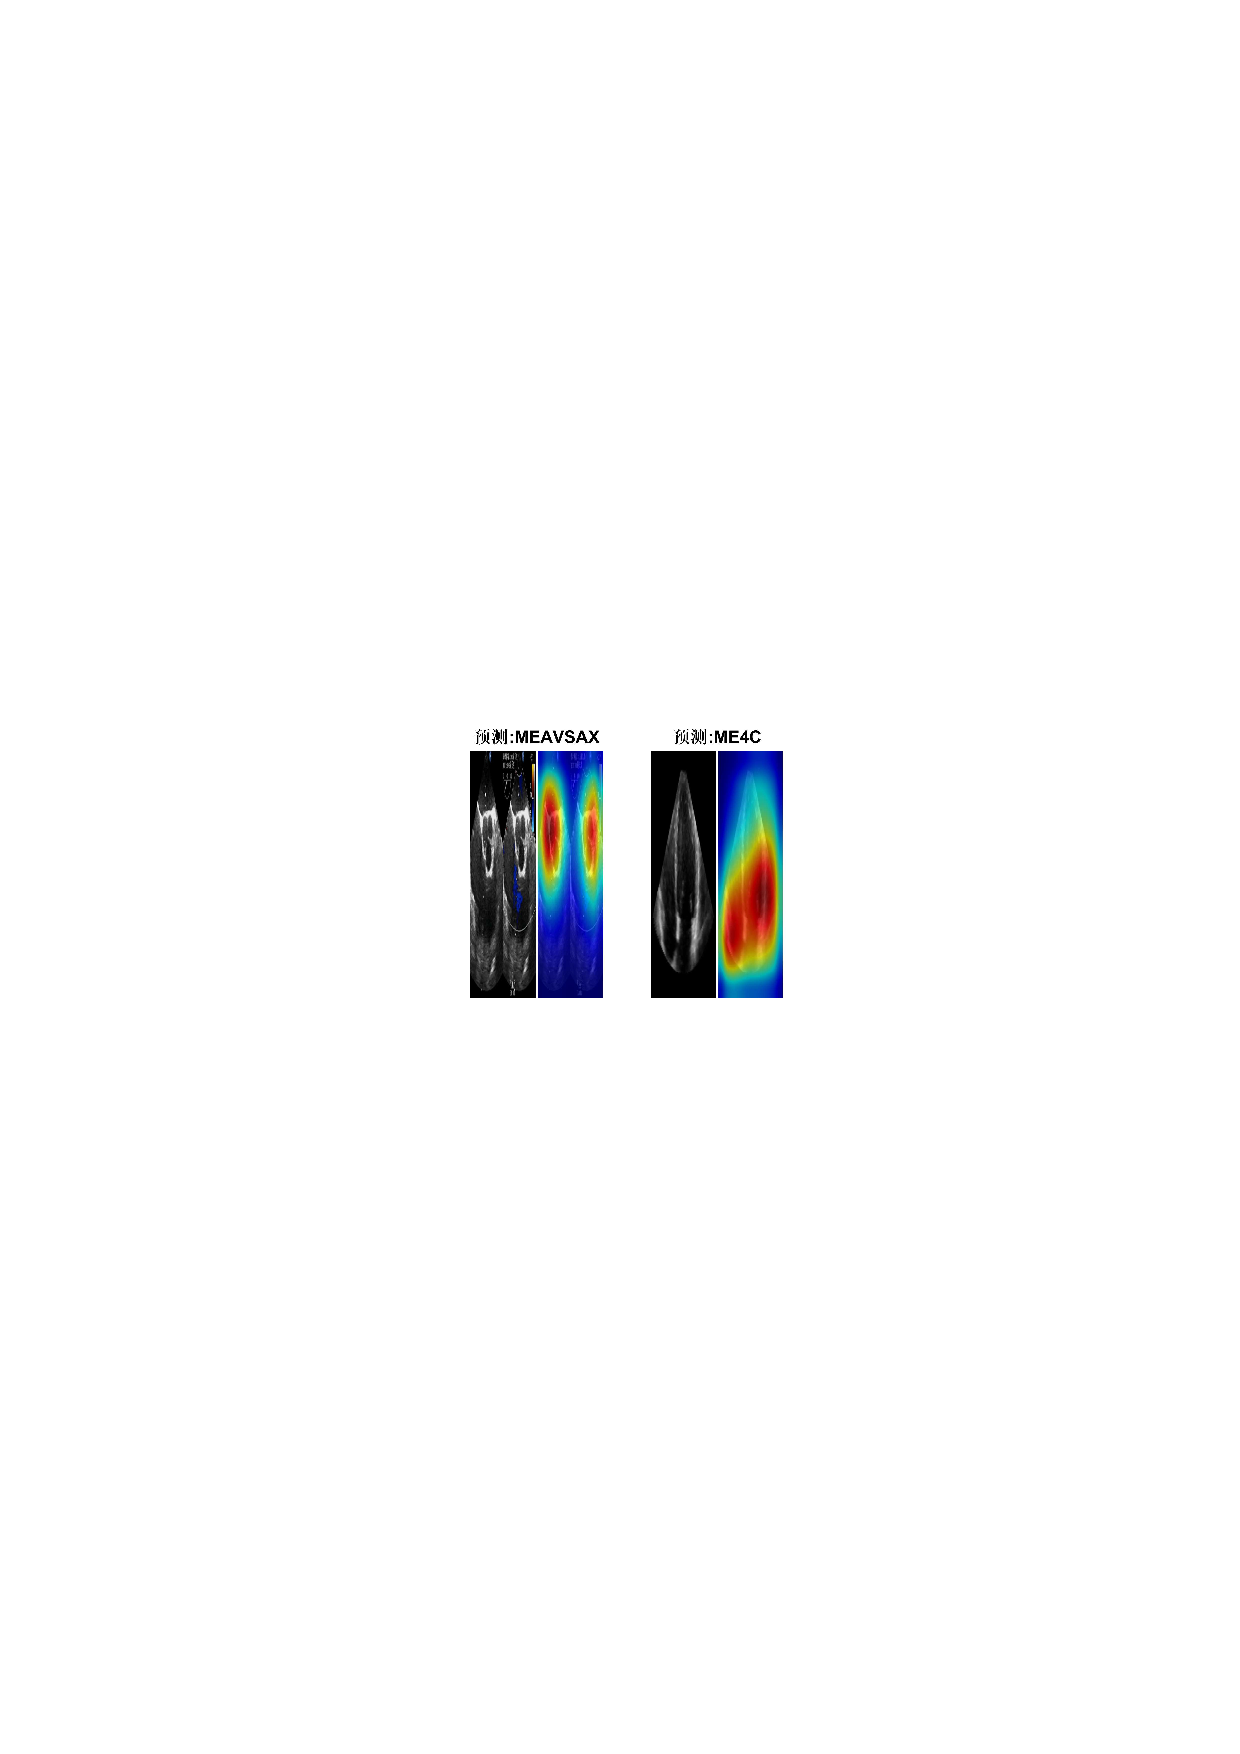
\includegraphics[width=0.85\textwidth,height=0.15\textheight]{ch03_06}
\caption{深度模型泛化性能可视化分析}
\label{fig:ch03_06}
\end{figure}  
  
深度模型泛化性能可视化结果如图\ref{fig:ch03_06}所示,原图像分别是带彩色多普勒的双扇形切面(图\ref{fig:ch03_06}a)和经胸的四腔心切面(图\ref{fig:ch03_06}b),这两个图是跟数据集中的经食道超声心动图差异较大,说明深度卷积网络模型确实能对标准切面进行语义分类, 表明模型确实能提取到高层语义的特征, 深度卷积网络泛化能力优异。图7中可视化结果也能很好的解释模型的有效性,如图\ref{fig:ch03_06}中显著性热力图红色区域图定位到图中的圆圈,也是医师认定该切面的关键性结构,图\ref{fig:ch03_06}b定位到左心室和右心室的边界等,都跟医师的决策判断依据是一致的。并且该方法也能作为判断学习模型是否有效的根据,不经过微调的模型虽然能得到较高的分类准确度,并不能得到类似的显著性热力图。

\section{小结与讨论}

本文提出了一种基于深度卷积神经网络的超声心动图标准切面自动识别方法,利用所述全局空间金字塔均值池化方法进行微调迁移学习,实验结果表明该方法识别准确率高,并实验分析了数据规模对模型分类精度的影响,结果表明基于深度卷积网络的识别方法应成为超声心动图自动识别的基准方法,接下来会探索更精细类别分类问题,如舒张末期和收缩末期标准切面的识别等。可视化深度模型的实验,对模型的可解释性和有效性进行了分析,推断深度模型的优异的分类性能和泛化能力的原因是可以对类别显著性区域进行判别,采用的可视化方法是对网络模型整体的理解,具体各层特征怎么耦合成语义信息仍需进一步探索。




